\chapter{Referencial Teórico}

Uma imagem pode ser definida por uma função bidimensional $f(x,y)$ onde $x$ e $y$ são um par de coordenadas espaciais e $f$ em qualquer par de coordenadas $(x,y)$ representa a intensidade da imagem naquele ponto. Quando $x,y$ e os valores das intensidades de $f$ são todos finitos e em quantidades discretas, pode-se dizer que a imagem é uma imagem digital. Os  elementos  constituintes das imagens são denominados \emph{pels} ou \emph{pixels} \cite{Gonzalez:2006:DIP:1076432}. A quantidade de \emph{pixels} nas dimensões de altura e largura indicam a resolução de uma imagem. A Figura \ref{andressa}, mostra um exemplo de imagem monocromática digital cuja resolução é de 390x390, é representada matricialmente na Figura \ref{matriz-andressa}. 


\begin{figure}[htb]
\begin{center}
  \caption{(a) Exemplo de imagem digital (b) Representação matricial da imagem.}
  \begin{subfigure}[b]{0.6\textwidth}
  \centering
      
\includegraphics[scale=0.6]{images/bw.png}
    \caption{}
    \label{andressa}
  \end{subfigure}
 %
  \begin{subfigure}[b]{0.6\textwidth}
  \centering
    \begin{center}
	%
	\sbox0{$\vcenter{\hbox{$\begin{bmatrix}
	0 & 0 & 0 & ...  & 0 & 0 \\ 
	0 & 0 & 0 &...  & 0 & 0\\ 
	\vdots & \vdots & \vdots & \vdots &  \vdots & \vdots \\ 
	0 & ... & 127 & ... & 0 & 0\\
	\vdots & \vdots & \vdots & \vdots &  \vdots & \vdots \\ 
	0 & 0 & 0 & ...  & 0 & 0
	\end{bmatrix}$}}$}%
	%
	$f(x,y)$ $=
	  \underbrace{\vrule width0pt depth \dimexpr\dp0 + .3ex\relax\copy0}_{w = 390}%
	  \left.\kern-\nulldelimiterspace
	    \vphantom{\copy0}
	  \right\rbrace \scriptstyle{h = 390}
	$
	\end{center}
    \caption{}
    \label{matriz-andressa}
  \end{subfigure}
  
  \legend{\textbf{Fonte:} \citeonline{Gonzalez:2006:DIP:1076432}.}
\end{center}

\end{figure}

O processamento digital de imagens (PDI) refere-se à utilização de métodos que manipulam imagens digitais e que geram como resultado outras imagens digitais. Apesar de a visão humana ser limitada ao espectro eletromagnético, dispositivos digitais podem operar em quase todo o espectro eletromagnético, realizando assim, operações com imagens geradas de origens não comuns aos humanos, como ultrassom e microscópio eletrônico. Sendo assim, a área de PDI engloba uma grande variedade de campos de aplicações \cite{Gonzalez:2006:DIP:1076432}.

\section{Aquisição de Imagens Digitais}
Em geral, a aquisição de imagens digitais é feita através de equipamentos digitais de captura de imagens como câmeras, por exemplo. Os dispositivos de captura possuem componentes sensíveis às ondas eletromagnéticas refletidas por objetos presentes em uma cena. Desta forma, uma imagem digital é gerada pela conversão de  dados analógicos em dados digitais. O processo executado por estes equipamentos é divido em três etapas: amostragem, quantização e codificação.

A amostragem é o processo responsável por converter coordenadas contínuas em  discretas \cite{albovik}. A quantização é a operação responsável por converter as intensidades de luz de cada ponto da imagem em uma representação numérica discreta \cite{widrow}. Uma vez que as etapas de amostragem e quantização são passadas, se faz necessário que os valores discretos obtidos na fase de quantização sejam codificados em sequências de bits para que assim possam ser considerados digitais. A Figura \ref{sq} apresenta graficamente as etapas envolvidas na aquisição de imagens digitais.

\begin{figure}[htb]
\begin{center}
  \caption{(a) Imagem contínua (b) Linha de varredura do ponto A a B (c) Amostragem e quantização (d) Linha de varredura digital.}
  \begin{subfigure}[b]{0.4\textwidth}
  \centering
      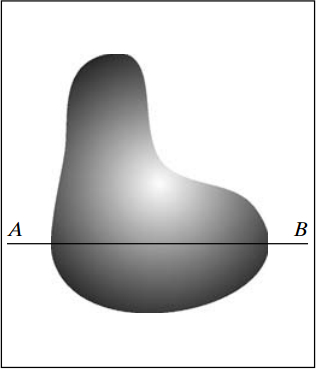
\includegraphics[scale=0.4]{images/sampling/image.jpg}
    \caption{}
    \label{imagemContinua}
  \end{subfigure}
 %
  \begin{subfigure}[b]{0.4\textwidth}
  \centering
    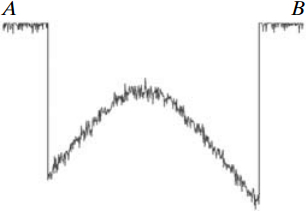
\includegraphics[scale=0.4]{images/sampling/sq.jpg}
    \caption{}
    \label{scanline}
  \end{subfigure}
  
  \begin{subfigure}[b]{0.4\textwidth}
  \centering
      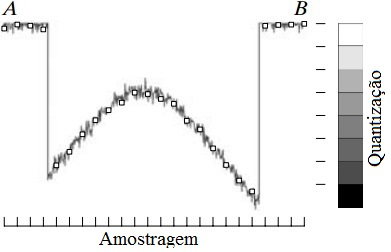
\includegraphics[scale=0.4]{images/sampling/sampling.jpg}
    \caption{}
    \label{sampling}
  \end{subfigure}
 %
  \begin{subfigure}[b]{0.4\textwidth}
  \centering
    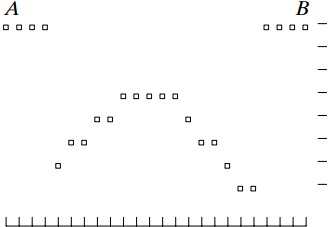
\includegraphics[scale=0.4]{images/sampling/quant.jpg}
    \caption{}
    \label{quant}
  \end{subfigure}
  \label{sq}
  \legend{\textbf{Fonte:} \citeonline{Gonzalez:2006:DIP:1076432}.}
\end{center}

\end{figure}


\begin{comment}
\textbf{A quantização é a operação responsável por converter uma quantidade física e contínua em uma representação numérica (não entendi).} Os valores contínuos são associados a valores discretos mais próximos possíveis a representação contínua. A quantização é semelhante a amostragem no sentido de discretizar valores, a diferença é que este processo acontece em cima dos valores de amplitudes obtidas no processo de amostragem \cite{widrow}. \textbf{--- Reescreva esse parágrafo - FEITO ACIMA}
\end{comment}



\section{Imagens Coloridas}
Estudos mostram que os sensores do olho humano podem ser divididos em três principais categorias que correspondem basicamente as cores vermelha, verde e azul \cite{fundamentalsofmultimedia}. Sendo assim, a literatura considera estas cores como sendo cores primárias. Isto significa que combinações destas cores geram outras cores \cite{fundamentalsofdigitalimageprocessing}. 

Como a área de PDI engloba processos que têm como entrada e saída imagens, diferentes sistemas de cores foram estudados para dar suporte ao processo de exibição de imagens de acordo com a limitação e especificidade de cada dispositivo de saída de imagens. São exemplos de dispositivos de saídas que necessitam de diferentes sistemas de cores a impressora, televisão colorida e dispositivos de plasma.

Em termos de PDI, os modelos de cores mais comuns são RGB (\emph{red, green, blue}) para monitores coloridos e uma grande parte de câmeras de vídeo colorido, CMY (\emph{cyan, magenta, yellow}) e CMYK (\emph{cyan, magenta, yellow, black}) para impressão colorida, e HSI (\emph{hue, saturation, intensity}) \cite{Gonzalez:2006:DIP:1076432}. O RGB representa o sistema de cores que usa as cores vermelho, verde e azul como cores primárias, o CMY as cores ciano, magenta e amarelo, o CMYK as cores do CMY com adição da cor preta, por fim o HSI que refere-se à tonalidade, saturação e intensidade.

No modelo RGB, cada cor aparece em seus componentes primários, vermelho, verde, e azul. Este modelo é baseado em um sistema de coordenadas cartesianas. O subespaço de cores é representado no cubo da Figura \ref{rgb-cube}. Neste modelo, a escala de cinza se estende desde o preto, na origem até o branco no canto mais distante da origem \cite{fundamentalsofmultimedia}.

\begin{figure}[htb]
\begin{center}
  \caption{(a) Esquema do cubo de cores RGB (b) Cubo de cores do RGB.}
  \begin{subfigure}[b]{0.4\textwidth}
  \centering
      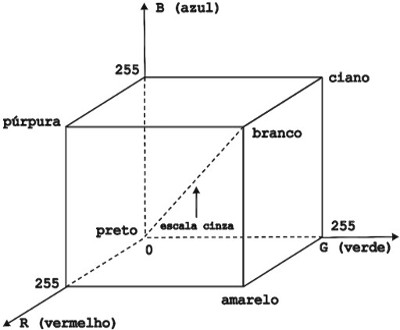
\includegraphics[scale=0.4]{images/rgb-cube.jpg}
    \caption{}
    \label{rgb-cube}
  \end{subfigure}
 %
  \begin{subfigure}[b]{0.4\textwidth}
  \centering
    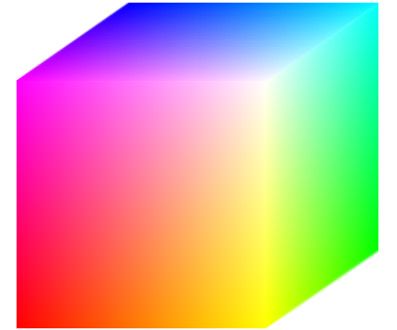
\includegraphics[scale=0.4]{images/rgb-color-cube.jpg}
    \caption{}
    \label{rgb-cube-full}
  \end{subfigure}
  
  \legend{\textbf{Fonte:} \citeonline{Gonzalez:2006:DIP:1076432}.}
\end{center}

\end{figure}

Como visto anteriormente, uma imagem monocromática é definida por uma função bidimensional $f(x,y)$ e pode ser representada computacionalmente por uma matriz bidimensional de forma que cada célula da matriz representa uma intensidade de cor da imagem. Sendo assim, uma imagem representada no sistema RGB possui três matrizes de forma que cada matriz representa as intensidades de cada cor deste sistema. Neste modelo, cada célula da matriz possui um valor que é representado por 8 bits que com a combinação de três cores permite a composição de $(2^8)^3$ = 16.777.216 cores.

As Figuras \ref{red}, \ref{green} e \ref{blue} representam a decomposição de uma imagem colorida nos três canais de cores do sistema RGB. Cada imagem representa a intensidade de uma respectiva cor na imagem. Sendo assim, a imagem colorida é formada pela combinação destas três imagens. A Figura \ref{coloridaAmpliada} é um exemplo de imagem colorida ampliada. Cada \emph{pixel} é descrito por uma combinação das três intensidades de cores.

\begin{figure}[htb]
\begin{center}
  \caption{Decomposição de imagem nos canais de cores do sistema RGB.}
  \begin{subfigure}[b]{0.4\textwidth}
  \centering
      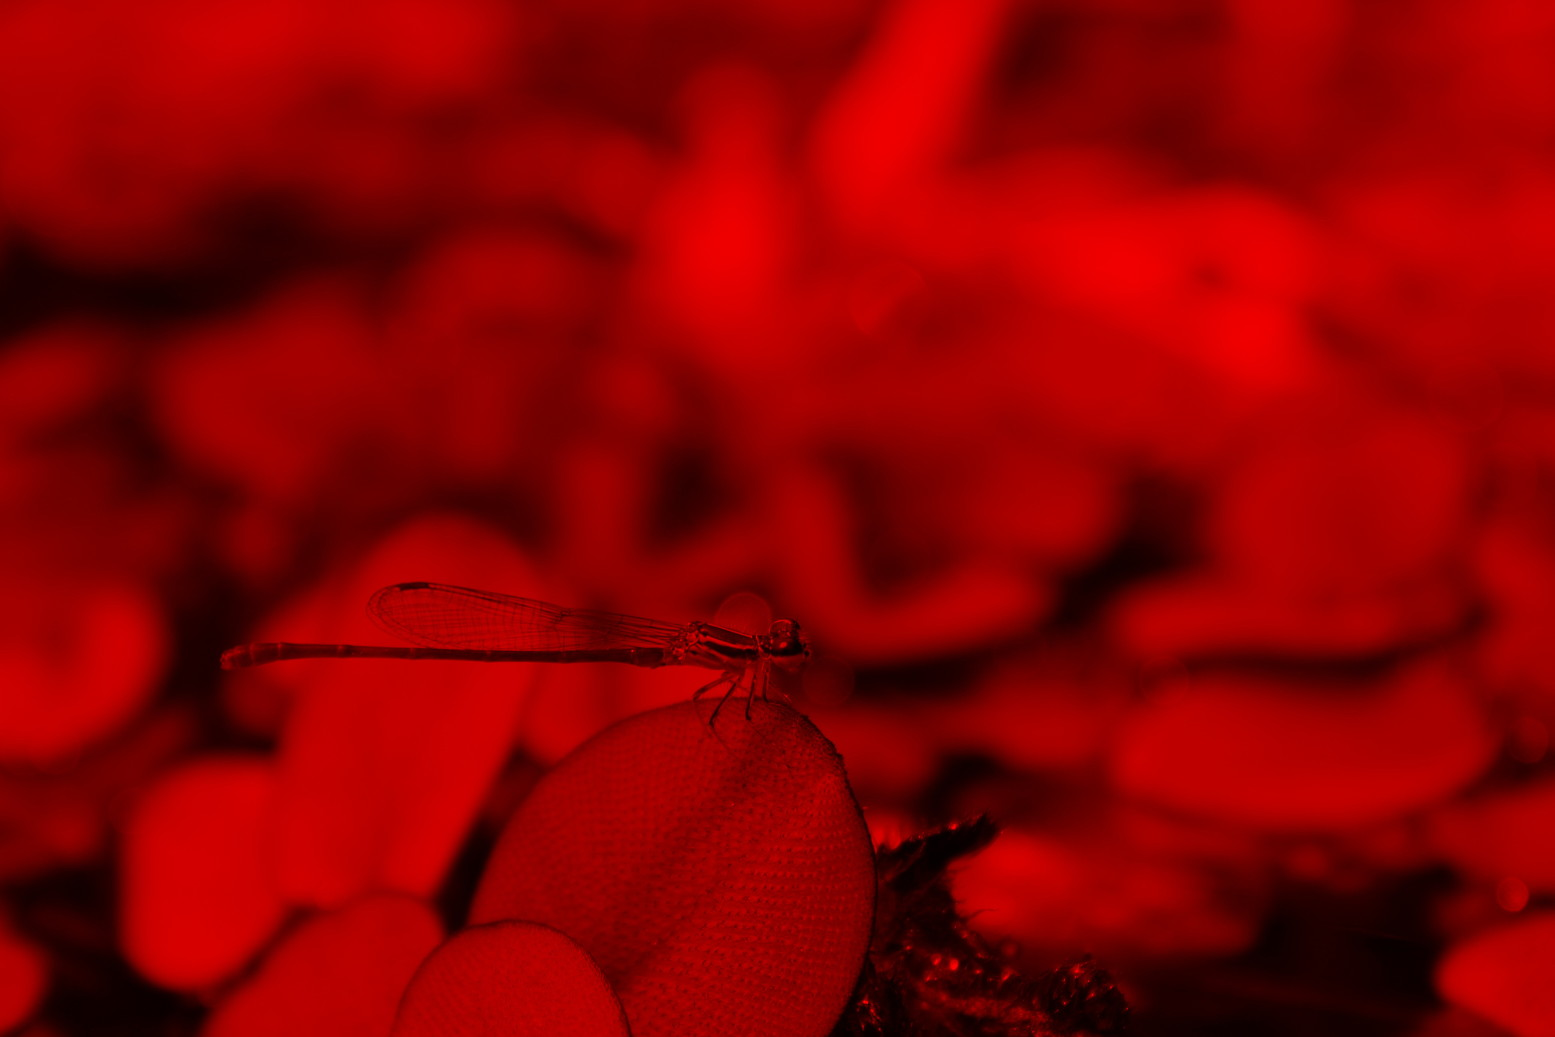
\includegraphics[scale=0.11]{images/red.JPG}
    \caption{Canal Vermelho}
    \label{red}
  \end{subfigure}
 %
  \begin{subfigure}[b]{0.4\textwidth}
  \centering
    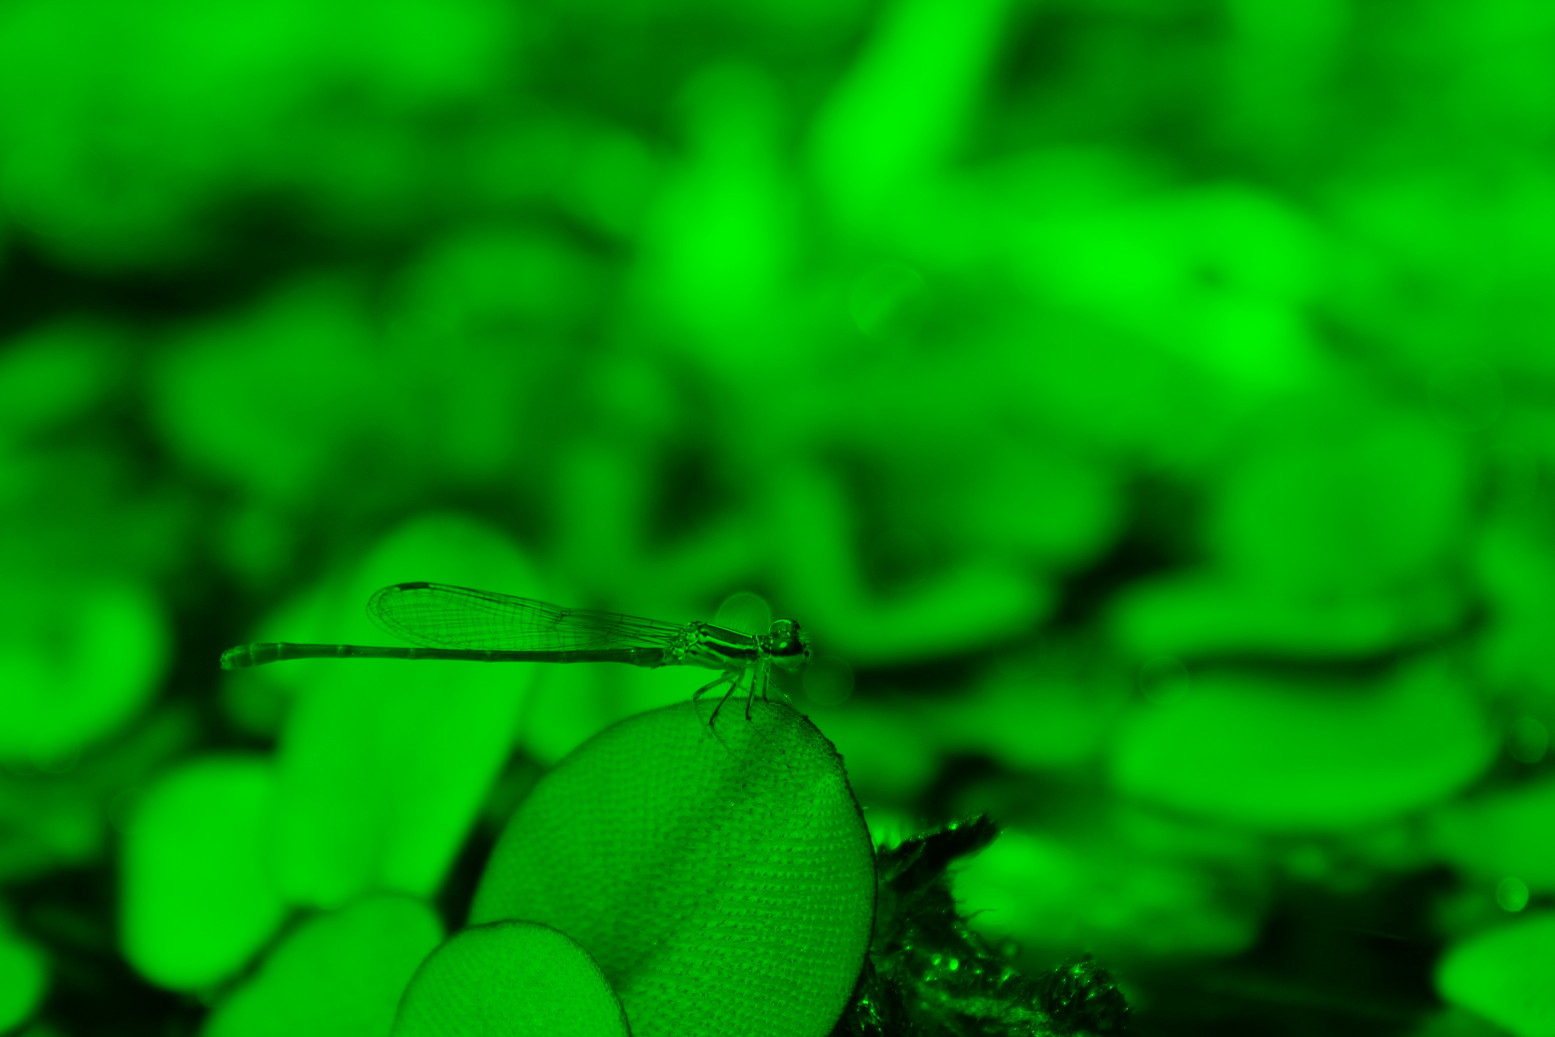
\includegraphics[scale=0.11]{images/green.JPG}
    \caption{Canal Verde}
    \label{green}
  \end{subfigure}
  
  \begin{subfigure}[b]{0.4\textwidth}
  \centering
    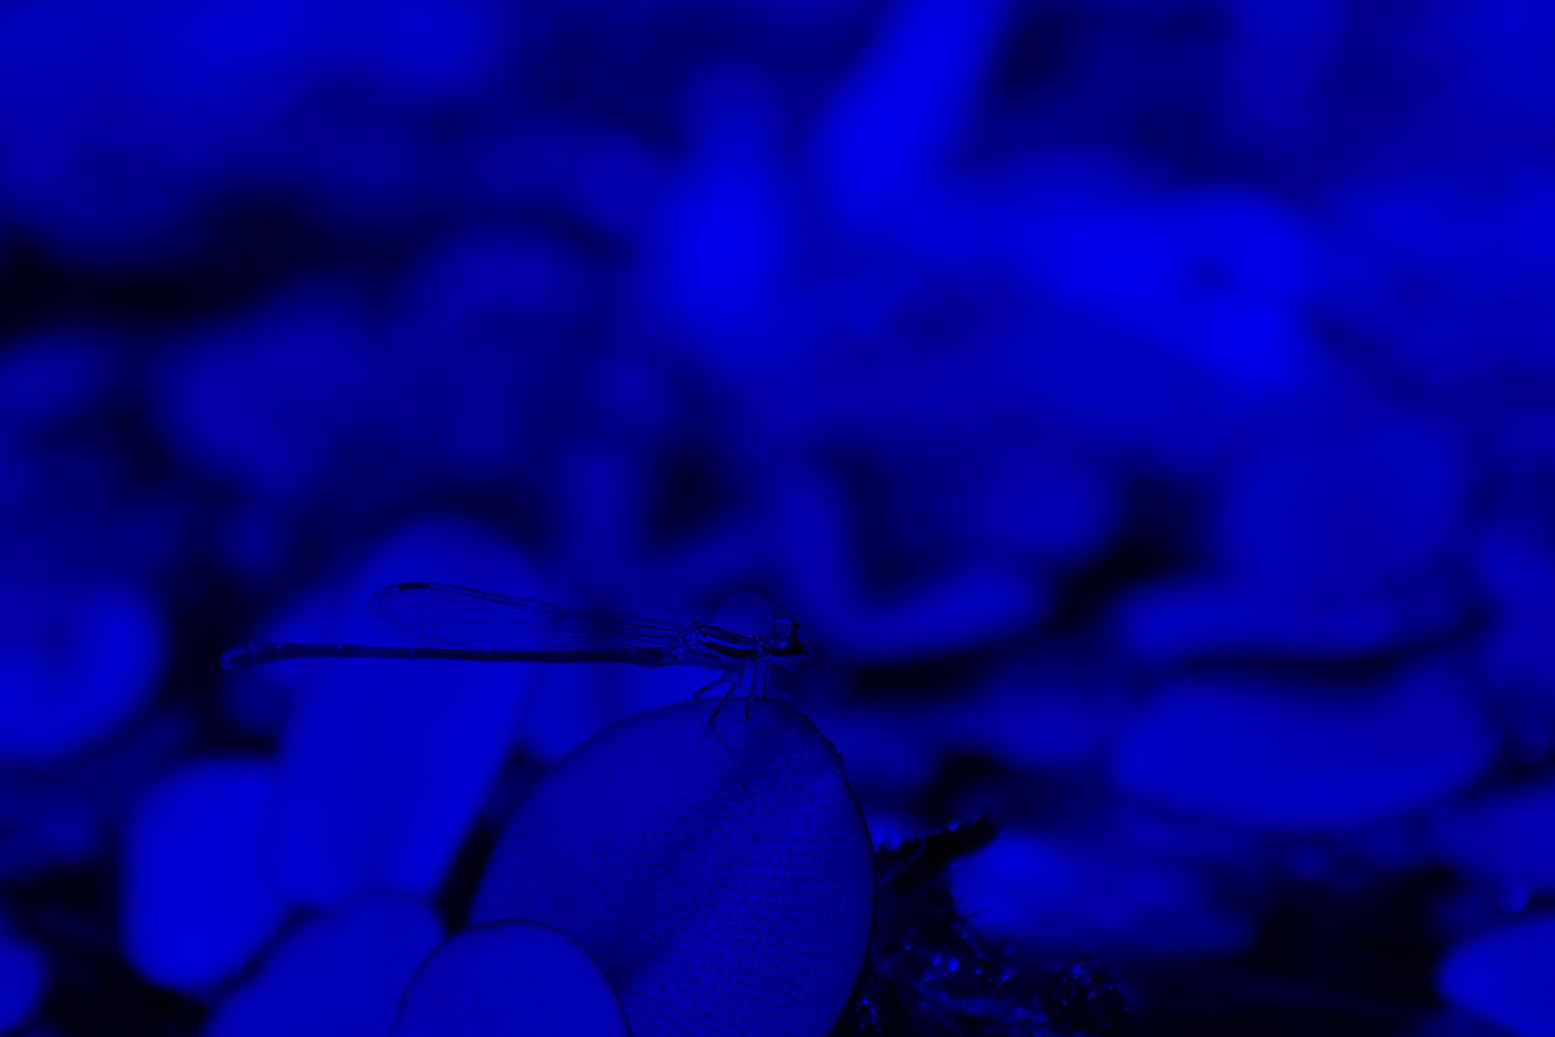
\includegraphics[scale=0.11]{images/blue.JPG}
    \caption{Canal Azul}
    \label{blue}
  \end{subfigure}
  
  \legend{\textbf{Fonte:} Autoria Própria.}
\end{center}

\end{figure}


\section{Descritores de Imagens Digitais}
Um descritor é uma representação resumida para a informação contida no interior da imagem. Dependendo do descritor utilizado, algumas características podem ser preservadas e outras perdidas. Na literatura existem e são propostos vários descritores de imagens: descritores de cores, textura e forma \cite{tuytelaars2008local, Gonzalez:2006:DIP:1076432}. Neste trabalho foram utilizados dois descritores, autovetor e histograma, que serão utilizados como critério de comparação entre as imagens. Estes descritores foram adotados por serem suficientes para representar as imagens sem que precisem ser complementados por outros descritores.

\begin{figure}[hb]
\begin{center}
  %\caption{Imagem colorida ampliada. \textbf{-- Explique que as cores estão representadas nos números em cada quadro da imagem}}
  %\begin{subfigure}[b]{0.6\textwidth}
  \centering
  \caption{Imagem colorida ampliada.}
      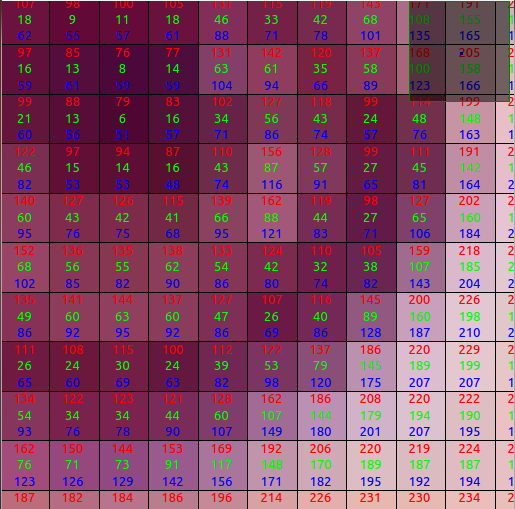
\includegraphics[scale=0.5]{images/lenaZoom.png}
    
    \label{coloridaAmpliada}
  %\end{subfigure}
  
  \legend{\textbf{Fonte:} \citeonline{montabone}.}
\end{center}

\end{figure}

\subsection{Autovetor}
Um vetor é uma grandeza com módulo, direção e sentido. Os vetores são representados por retas que ligam dois pontos. O ponto que define a ponta da reta é chamado de ponto final e o outro ponto é chamado de ponto de origem. 

O autovetor de uma matriz quadrada $A_{n \times n}$ é um vetor $v$ que atende a Equação \ref{autovetor} onde $\lambda \in \mathbb{R}$ é o autovalor de $A$ \cite{boldrini}. Quando $A_{n \times n}$ é uma imagem, o autovetor dominante mantém os aspectos mais efetivos da imagem de forma que $v$ indica a direção de maior variação da informação, neste caso a informação de cor.

\begin{equation}
  \label{autovetor}
  	Av = \lambda v
\end{equation}

\begin{comment}
\textbf{Explicar o que é um autovetor de uma matriz. Coloque a equação. Cite livros de álgebra aqui. Explique que o autovetor dominante indica a direção de maior variação da informação, neste caso a informação de cor}
\end{comment}

Os autovetores são vetores representados por um ponto de origem na origem do espaço e um ponto final que é calculado através do método das potências. O método das potências é um método iterativo aplicado a uma matriz quadrada $A_{n \times n}$ que produz uma sequência de vetores $v_i$ que convergem ao autovetor dominante. O método das potências é apresentado por \citeonline{yousef} e \citeonline{ping} e é exibido no {Algoritmo \ref{power}}.

\begin{algorithm}[H]
\caption{Método das potências.}
\label{power}
	\begin{algorithmic}[1]
	\LeftTextComment{Seja $v_0$ um vetor não nulo.}
		\For{$ i \gets 0, 1, 2, ...$ até convergir }
				\State $v_{i+1} \gets Av_i$
				\State $v_{i+1} \gets \frac{v_{i+1}}{\parallel v_{i+1} \parallel}$
		\EndFor
	\end{algorithmic}
\end{algorithm}

A distância calculada entre duas imagens representadas por autovetores $v$ e $w$ é feita com base no ângulo entre estes vetores. \citeonline{boldrini} mostra que o ângulo entre dois vetores é calculado através da Equação \ref{angulo}.

\begin{equation}
  \label{angulo}
  	\theta = arccos \Bigg ( \frac{\langle v, w \rangle}{\parallel v \parallel \parallel w \parallel} \Bigg )
\end{equation}

\subsection{Histograma}

O histograma de uma imagem digital $A_{n \times m}$ é a função discreta $h(r_k) = n_k$, de forma que $r_k$ são os valores de intensidades da imagem e $n_k$ é o número de \emph{pixels} na imagem com intensidade $r_k$. O histograma pode ser normalizado através da divisão de cada componente pelo número total de \emph{pixels} da imagem $n \times m$. Sendo assim, um histograma normalizado é denotado por $p(r_k) = n_k/{nm}$ de forma que $p(r_k)$ representa a probabilidade de ocorrência da intensidade $r_k$ \cite{Gonzalez:2006:DIP:1076432}.

A visualização gráfica de um histograma se dá através da relação entre $h(r_k) = n_k$ e $r_k$ ou $p(r_k) = n_k/{nm}$ e $r_k$ como apresenta a Figura \ref{histogramas}. A representação gráfica de um histograma pode ser utilizada para analisar características visuais da imagem e possivelmente identificar particularidades na imagem, como identificar as cores predominantes ou o nível de contraste.

Na Figura \ref{escura} os componentes do histograma estão concentrados no lado esquerdo da escala de intensidade que representa os baixos níveis de intensidade. Semelhantemente, os componentes do histograma da Figura \ref{clara} tendem à direção do lado direito da escala. A Figura \ref{baixoContraste} com baixo contraste tem um histograma graficamente estreito que concentra as ocorrências das intensidades ao centro. Já na Figura \ref{altoContraste}, os componentes do histograma são distribuídos de maneira mais uniforme.

A distância entre dois histogramas $x$ e $y$ é calculada utilizando a distância euclidiana que é usada para calcular distâncias no $\mathbb{R}^n$. A distância euclidiana é apresentada na Equação \ref{distanciaEuclidiana} \cite{deza}.

\begin{equation}
  \label{distanciaEuclidiana}
  d(x,y) = \sqrt{ (x_1 - y_1)^2 + ... + (x_n - y_n)^2 }
\end{equation}

\begin{figure}[h]
\begin{center}
  \caption{Quatro tipos básicos de imagem: escura, clara, baixo contraste, alto contraste e seus histogramas correspondes.}
  \begin{subfigure}[b]{0.49\textwidth}
  \centering
      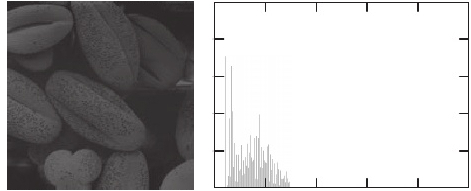
\includegraphics[scale=0.45]{images/escura.jpg}
    \caption{Escura}
    \label{escura}
  \end{subfigure}
 %
  \begin{subfigure}[b]{0.49\textwidth}
  \centering
    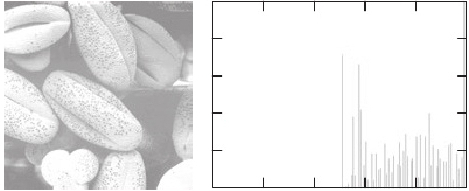
\includegraphics[scale=0.45]{images/clara.jpg}
    \caption{Clara}
    \label{clara}
  \end{subfigure}
  
  \begin{subfigure}[b]{0.49\textwidth}
  \centering
    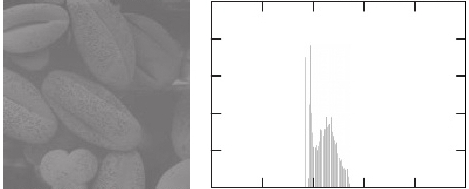
\includegraphics[scale=0.45]{images/baixoContraste.jpg}
    \caption{Baixo Contraste}
    \label{baixoContraste}
  \end{subfigure}
  %
  \begin{subfigure}[b]{0.49\textwidth}
  \centering
    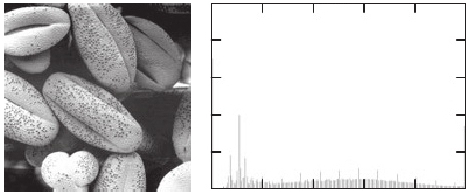
\includegraphics[scale=0.45]{images/altoContraste.jpg}
    \caption{Alto Contraste}
    \label{altoContraste}
  \end{subfigure}
  
  \label{histogramas}
  \legend{\textbf{Fonte:} \citeonline{Gonzalez:2006:DIP:1076432}.}
\end{center}

\end{figure}

%\textbf{Faltou explicar quem são x e y}

% -  \textbf{trocar clustering por agrupamento no texto todo}

\section{Agrupamento}
Agrupamento é o nome dado ao processo de agrupar ou categorizar elementos. Este processo tem como entrada um conjunto de elementos sem organização prévia e busca identificar possíveis grupos de elementos que se assemelham entre si. Sendo assim, elementos semelhantes tendem a ser alocados nos mesmos grupos e consequentemente elementos distintos tendem a ficar em grupos distintos \cite{carvalho}. 

%------------{Os grupos resultantes deste processo representa o  de uma forma sintetizada informações a respeito dos elementos.-----------------

Os grupos identificados neste processo também podem ser chamados de \emph{clusters}. O processo de identificação dos \emph{clusters} pode ser chamado de clusterização.

A clusterização de um conjunto de elementos pode acontecer de maneira supervisionada e não-supervisionada. O processo de clusterização supervisionado requer a intervenção humana enquanto que a clusterização não supervisionada não requer a intervenção humana. O algoritmo de agrupamento por nuvens dinâmicas usado neste trabalho se encaixa no grupo de algoritmo de clusterização não supervisionado.

As estratégias de clusterização podem ser divididas em dois tipos principais: hierárquicos e particionais. Os algoritmos hierárquicos são divididos em aglomerativos e divisivos. Os algoritmos hierárquicos organizam os conjuntos de dados em estruturas hierárquicas denominadas de dendogramas e com isso aplicam sucessivas divisões dos elementos \cite{leandro}.

\begin{comment}
\tikzstyle{every node}=[draw=black,thick,anchor=west]
\tikzstyle{selected}=[draw=red,fill=red!30]
\tikzstyle{optional}=[dashed,fill=gray!50]

\begin{figure}
\centering

\begin{tikzpicture}[%
  grow via three points={one child at (0.5,-0.7) and
  two children at (0.5,-0.7) and (0.5,-1.4)},
  edge from parent path={(\tikzparentnode.south) |- (\tikzchildnode.west)}]
  \node {Clusterização}
    child { node {Hierárquico}
    	child { node {Aglomerativo}}
        child { node {Divisivo}}
    }	
    child [missing] {}				
    child [missing] {}	
    child { node {Particional}};
\end{tikzpicture}
\caption{Classificação das estratégias de clusterização} \label{tipos_clustering}
\end{figure}

\end{comment}

As estratégias de agrupamentos particionais buscam dividir um conjunto de elementos de entrada em um número fixo de \emph{clusters}. Estas estratégias utilizam pontos que se localizam no mesmo espaço dimensional dos elementos para representar cada um dos grupos formados \cite{leandro}. Estes pontos são denominados de protótipos e são usados como parâmetro de distância de um elemento ao \emph{cluster}.

\subsection{Agrupamento por Nuvens Dinâmicas}

O algoritmo de agrupamento por nuvens dinâmicas é um algoritmo iterativo de agrupamento particional que itera sobre passos de alocação de elementos e representação de \emph{clusters} até que o critério de parada seja alcançado.

O problema de otimização resolvido por este algoritmo é definido por \citeonline{carvalho} como se segue. Seja $\Omega$ o conjunto de $n$ objetos indexados por $i = 1, ..., n$ e descritos por $p$ variáveis quantitativas. Cada objeto $i$ é descrito por um vetor $\mathrm{x}_i = (x{^1_i}, ..., x{^p_i}) \in \Re^p$. O problema é achar a partição $P = (C_1, ..., C_k)$ de $\Omega$ em $K$ \emph{clusters} e o conjunto $Y = (y_1, ..., y_K)$ de exemplares que minimizam o critério de particionamento $g(P,Y)$ que mede a adequação entre os \emph{clusters} e seus representantes.

A inicialização do algoritmo se dá pela declaração inicial das partições e de seus respectivos protótipos como mostra o Algoritmo \ref{initialize}. Uma vez inicializado, o algoritmo busca encontrar a melhor alocação para os elementos de maneira que o critério de particionamento $g(P,Y)$ seja minimizado. Para tal, os elementos são alocados nos \emph{clusters} de acordo com suas proximidades aos exemplares \cite{carvalho}.

\begin{algorithm}[htb]
\caption{Função \emph{Initialize} que inicializa os \emph{K clusters}.}
\label{initialize}
	\begin{algorithmic}[1]
		\Function{initialize}{}
			\LeftTextComment{Escolha uma partição $(C_1, ..., C_K)$ de $\Omega$ ou escolha $K$ objetos diferentes $y_1, ..., y_K$ entre $\Omega$ e aloque cada objeto $i$ ao exemplar mais próximo para construir a partição inicial $(C_1, ..., C_K)$.			
			}
		\EndFunction
	\end{algorithmic}
\end{algorithm}

O Algoritmo \ref{representation} mostra que a eleição dos protótipos acontece através da verificação de qual elemento está mais próximo ao restante dos elementos, este elemento representará o centro do \emph{cluster} e por isso pode ser chamado de centroide. Em algumas configurações do algoritmo, o representante do \emph{cluster} pode ser calculado como a média de todos os elementos presentes naquele \emph{cluster}. O centroide de um \emph{cluster} poderá ser usado como parâmetro para o cálculo de distância de um elemento ao \emph{cluster}.

\begin{algorithm}[htb]
\caption{Função \emph{Representation} que elege os protótipos de cada \emph{cluster}.}
\label{representation}
	\begin{algorithmic}[1]
		\Function{representation}{}
			\For{$ k \gets 0; i<K; k++ $}
				\LeftTextComment{Calcule o exemplar $y_k$ }
			\EndFor			
		\EndFunction
	\end{algorithmic}
\end{algorithm}

O Algoritmo \ref{allocation} apresenta a função responsável por alocar os elementos em seus respectivos \emph{clusters}. Esta etapa do algoritmo de agrupamento por nuvens dinâmicas percorre todos os elementos averiguando o \emph{cluster} em que o elemento melhor se encaixa (menor distância) para que a melhor configuração seja estabelecida.

\begin{algorithm}[htb]
\caption{Função \emph{Allocation} que aloca os elementos.}
\label{allocation}
	\begin{algorithmic}[1]
		\Function{Allocation}{}
			\State $teste \gets 0$
			\For{$ i \gets 0; i<n; i++ $}
					\LeftTextComment{seja o \emph{cluster} $C_{k*}$ tal que $k* = min_{k=0,...,K} \ d^{k}_r (\mathrm{x}_i, \mathrm{y}_k)$}
					\If{$i \in C_k \quad E \quad k* \neq k $}
						\State $teste \gets 1$
						\State $C_{k*} \gets C_{k*} \cup \{i\}$
						\State $C_k \gets C_k \setminus \{i\}$
					\EndIf	
			\EndFor
			\State \Return \emph{teste}
		\EndFunction
	\end{algorithmic}
\end{algorithm}

A linha 2 do Algoritmo \ref{allocation} declara a variável que indica quando uma mudança na configuração dos \emph{clusters} for efetivada. Esta mudança é essencial para o algoritmo de agrupamento por nuvens dinâmicas, uma vez que esta indicará a necessidade de mais uma iteração do algoritmo.

O Algoritmo \ref{dynamicClustering} reúne as etapas apresentadas para contemplar a proposta do algoritmo de agrupamento. Uma vez que os \emph{clusters} são inicializados, o algoritmo itera pelas etapas de representação (\Call{Representation}{}) e alocação (\Call{Allocation}{}) até que nenhuma melhoria possa ser feita pela etapa de alocação.

\begin{algorithm}[htb]
\caption{Algoritmo de agrupamento por nuvens dinâmicas.}
\label{dynamicClustering}
	\begin{algorithmic}[1]
		\Function{dynamicClustering}{}
		
			\State $\Call{initialize}{}$
			\Repeat
				\State $\Call{representation}{}$
				\State $teste \gets \Call{allocation}{}$
			\Until {\emph{teste = 0}}
		\EndFunction
	\end{algorithmic}
\end{algorithm}

\section{Internet}
O avanço e estruturação das redes de computadores possibilitaram que várias aplicações que se baseiam na comunicação em redes surgissem. A \emph{INTERNET} refere-se a arquitetura de redes globais que estão interconectadas e se comunicam através de conjuntos de regras e protocolos. A \emph{INTERNET} usa funcionalidades relativamente simples com escalabilidade, eficiência e utilidade suficientes para resultarem em um espaço confiável \cite{www}.

A \emph{World Wide Web} (WWW) ou simplesmente \emph{Web} é uma das diversas aplicações de escala mundial que possibilitam que instituições e pessoas de todo o mundo estejam conectadas através da \emph{INTERNET}.

A \emph{World Wide Web} pode ser considerada um enorme sistema para acessar documentos ligados, que consiste em milhões de clientes e servidores. Servidores mantêm conjuntos de documentos, enquanto clientes fornecem a usuários uma interface de fácil utilização para apresentar e acessar esses documentos \cite{distribuidostanenbaum}.

O padrão \emph{Web} teve início no Laboratório Europeu de Física Nuclear (\emph{European Particle Physics Laboratory} - CERN), em Genebra, como um projeto que permitiria seu grupo de pesquisadores, numeroso e geograficamente disperso, acessar documentos compartilhados por meio de um sistema simples de hipertexto. Um documento podia ser qualquer coisa que pudesse ser representada no terminal do computador de um usuário \cite{distribuidostanenbaum}. 

O núcleo de um site \emph{Web} é formado por um processo que tem acesso a um sistema de arquivos local que armazena documentos. O modo mais simples de referenciar um documento é por meio de uma referência denominada localizador uniforme de recurso ou \emph{Uniform Resource Locator} (URL) \cite{distribuidostanenbaum}. Cada documento disponível na \emph{Web} possui um URL associado que será usado para que o serviço cliente tenha acesso a estes documentos.

A comunicação entre um \emph{browser} e um servidor se baseia no protocolo de transferência de hipertexto ou \emph{Hypertext Transfer Protocol} (HTTP). O protocolo HTTP foi originalmente projetado para transferência de conteúdo \emph{Web}, mas agora suporta a transferência de arquivos de qualquer tipo \cite{fundamentalsofmultimedia}.

O \emph{browser} ou navegador é a aplicação responsável por abstrair os procedimentos envolvidos na requisição e tratamento da resposta obtida. A Figura \ref{http} ilustra o procedimento em que um cliente realiza uma requisição HTTP e obtém uma resposta do servidor. Uma vez que a máquina cliente recebe uma resposta do servidor com o conteúdo esperado, o \emph{browser} analisa a resposta e apresenta o conteúdo do documento.

\begin{figure}[htb]
\begin{center}
  \centering
  \caption{Organização global de \emph{Website}.}
      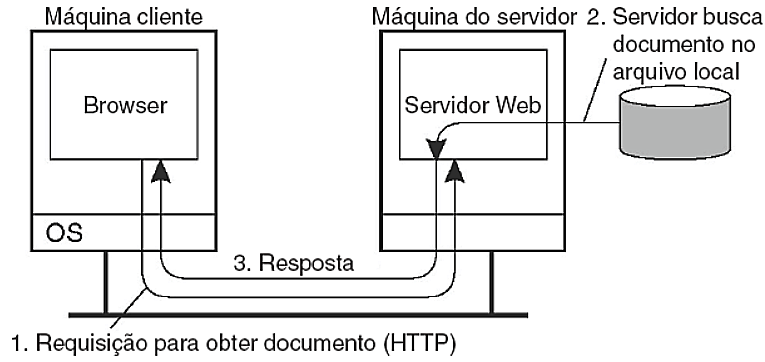
\includegraphics[scale=0.6]{images/httpTanenbaum.png}
    
    \label{http}
  %\end{subfigure}
  
  \legend{\textbf{Fonte:} \citeonline{distribuidostanenbaum}.}
\end{center}

\end{figure}

%O conteúdo de uma resposta HTTP contém essencialmente trechos que demarcam e descrevem a estrutura de uma página \emph{Web}, estilo e comportamento. 
 
\subsection{HTML e CSS}
Uma página \emph{Web} é formada principalmente de código HTML, uma linguagem de marcação usada para indicar ao \emph{browser} como estruturar as páginas. HTML consiste em uma série de elementos usados para delimitar ou marcar diferentes partes do conteúdo para que sejam exibidos de maneira específica de acordo com o elemento indicado \cite{mdn}. Os elementos são delimitados por \emph{tags} que definem o início de um elemento no formato \emph{<tag>} e \emph{</tag>} que delimita o fim do elemento. 

Um documento HTML simples é dividido entre cabeçalho e corpo. O cabeçalho descreve as definições do documento que são interpretadas antes do processo de montagem do documento ser concluído. Estas definições incluem título da página, \emph{links} para recursos utilizados e outras informações que o autor desejar especificar. O corpo de uma página descreve a estrutura do documento e seu conteúdo. Estas estruturas podem ser parágrafos, tabelas, formulários, listas de itens e botões \cite{fundamentalsofmultimedia}.

O Código \ref{exemploHtml} mostra o exemplo de uma página simples HTML. As linhas 1 e 10 delimitam que o texto em seu interior é um código HTML, as 2 e 4 delimitam o cabeçalho da página, as 6 e 9 delimitam o corpo. No interior destes elementos, a linha 3 declara o título da página, a linha 7 declara o título do texto e a linha 8 declara um parágrafo. O resultado deste exemplo em um \emph{browser} é apresentado na Figura \ref{htmlExemploImagem}.

\lstinputlisting[caption={Exemplo de página HTML}, label={exemploHtml},language=HTML]{code/htmlExample.html}


Os elementos HTML podem conter atributos que adicionam informações extras sobre o elemento. Um atributo permite que um elemento específico passe a ter uma identificação que pode ser usada para estilizar este elemento. A estilização de uma página e de seus elementos é feita através da linguagem \emph{Cascading Style Sheets} (CSS). A linguagem CSS permite a customização de cores de texto e fundo dos elementos, fontes, tamanhos e espaçamentos entre \mbox{outros \cite{mdn}}.

\begin{figure}[htb]
\begin{center}
  \centering
  \caption{Código \ref{exemploHtml} apresentado no \emph{browser}.}
      \fbox{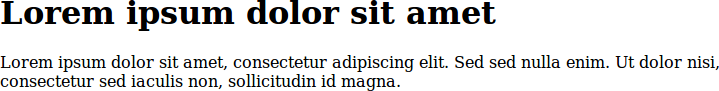
\includegraphics[scale=0.6]{images/htmlExemplo.png}}
    
    \label{htmlExemploImagem}
  
  \legend{\textbf{Fonte:} Autoria Própria.}
\end{center}

\end{figure}

\subsection{JavaScript} 
Os \emph{browsers} não se limitam apenas a apresentar as páginas \emph{Web} estáticas, eles permitem que os usuários interajam com páginas através da linguagem \emph{JavaScript}. Apesar do nome, \mbox{\emph{JavaScript}} e \emph{Java} são linguagens totalmente diferentes. A linguagem \emph{JavaScript} é uma linguagem de \emph{script} que é interpretada por um \emph{browser}, isto significa que os \emph{scripts} \emph{JavaScript} são executados por a máquina cliente sem a necessidade de passar por um compilador.\footnote{\emph{Script} é uma sequência de instruções a ser interpretada por um programa em vez de ser compilada.}

\emph{JavaScript} é uma linguagem de programação que permite a implementação de interações complexas nas páginas \emph{Web}. Ela permite a atualização de componentes HTML e regras CSS de maneira dinâmica e permite armazenar valores em variáveis, realizar operações em textos e executar ações em resposta a eventos que venham a acontecer na página \cite{mdn}. 

O Código \ref{exemploHtmlJS} é um exemplo de como \emph{JavaScript} pode interagir com HTML e CSS. Neste exemplo, o botão definido na linha 5 define o código \emph{JavaScript} a ser executado quando um evento de clique for detectado no botão. A ação declarada no atributo \emph{onclick} do botão HTML (\emph{document.getElementById('paragrafo').style.display = 'none'}) acessa o elemento HTML da linha 4 através do identificador definido no atributo \emph{id} e altera o atributo CSS \emph{display} para \emph{none} fazendo com que este fique invisível.

\lstinputlisting[caption={Exemplo de página HTML com código \emph{JavaScript} interagindo com CSS}, label={exemploHtmlJS},language=HTML]{code/htmlJavaScript.html}

Os códigos \emph{JavaScript} são executados por um processador de código \emph{JavaScript} contido no \emph{browser} depois que os códigos HTML e CSS são carregados. Isto porque os \emph{scripts} \emph{JavaScript} interagem com os componentes da página e precisam que eles estejam carregados.
 
\subsection{Disposição e Recuperação de Informações na Internet}
É fato que a \emph{Web} é um serviço democrático e dinâmico assim como o mundo virtual em geral. Com a popularização da \emph{INTERNET} e dos dispositivos digitais, artefatos multimídias dos mais diversos formatos são gerados a cada instante. Com isso, é comum que estas mídias sejam disponibilizadas na \emph{WWW} em \emph{Websites} dos mais diversos tipos.

Com o alto volume de dados sendo disponibilizados na \emph{INTERNET} nos mais variados formatos, a tarefa de encontrar ou recuperar uma informação de maneira não metódica é inviável pois os documentos disponibilizados não seguem qualquer ordem. É por isso que vários serviços como \emph{Google}, \emph{Yahoo} e \emph{Bing} se dispõem a realizar buscas na \emph{INTERNET} de maneira eficiente. O \citeonline{nms} indica que o motor de busca do \emph{Google} dominou cerca de 73\%  deste mercado.

O \emph{Google} é uma corporação dos Estados Unidos cuja missão é dominar o enorme volume de informações: ``\emph{organizar as informações do mundo e torná-las universalmente acessíveis e úteis}'' \cite{google}. 

Inaugurada em 1998, o \emph{Google} cresceu até ter uma fatia dominante do mercado de pesquisa na \emph{INTERNET} principalmente devido à eficiência de seu algoritmo. Desde seu sistema de produção inicial, até lidar com mais de 88 bilhões de pesquisas por mês (em 2010), seu principal mecanismo de busca nunca sofreu uma interrupção em todo esse tempo e seus usuários podem esperar resultados de consulta em torno de 0,2 segundos \cite{coulouris}.

A seguir é apresentada uma síntese de uma breve apresentação do serviço de busca do \emph{Google} feita por \citeonline{coulouris}. A função do mecanismo de busca do Google, assim como para qualquer mecanismo de pesquisa na \emph{Web}, é receber determinada consulta e retornar uma lista ordenada com os resultados mais relevantes que satisfazem essa consulta, pesquisando o conteúdo na \emph{Web}. O mecanismo de busca do \emph{Google} consiste em um conjunto de serviços para esquadrinhar a \emph{Web} e indexar e classificar as páginas descobertas. 

A tarefa de esquadrinhar refere-se a uma análise minuciosa do conteúdo da \emph{Web}. Esta tarefa analisa as páginas recursivamente coletando todos os \emph{links} que apontam para outras páginas para que estas também sejam esquadrinhados por este procedimento. O objetivo é mapear todo o conteúdo disponível na \emph{INTERNET} para que seja gerado um índice de palavras ou termos que serão usados como parâmetros de busca.

O índice de palavras gerado adota critérios de comparação e ordenação como número de ocorrências, posição no documento e tamanho da fonte usada. Além do índice de palavras, o motor de busca mantém um índice de \emph{links} que monitora as páginas que ligam a um determinado \emph{Website}. Este índice de \emph{links} é usado por o algoritmo \emph{PageRank} que classifica as páginas de acordo com sua relevância. 

%\subsection{Recuperação de Imagens}

%\subsubsection{Motores de Busca}

%\subsubsection{Google}



%\subsection{Aplicação}

